%%%%%%%%%%%%%%%%%%%%%%%%%%%%%%%%%%%%%%%%%
% Jacobs Landscape Poster
% LaTeX Template
% Version 1.1 (14/06/14)
%
% Created by:
% Computational Physics and Biophysics Group, Jacobs University
% https://teamwork.jacobs-university.de:8443/confluence/display/CoPandBiG/LaTeX+Poster
% 
% Further modified by:
% Nathaniel Johnston (nathaniel@njohnston.ca)
%
% This template has been downloaded from:
% http://www.LaTeXTemplates.com
%
% License:
% CC BY-NC-SA 3.0 (http://creativecommons.org/licenses/by-nc-sa/3.0/)
%
%%%%%%%%%%%%%%%%%%%%%%%%%%%%%%%%%%%%%%%%%

%----------------------------------------------------------------------------------------
%	PACKAGES AND OTHER DOCUMENT CONFIGURATIONS
%----------------------------------------------------------------------------------------

\documentclass[final]{beamer}

\usepackage[scale=1.24]{beamerposter} % Use the beamerposter package for laying out the poster

\usetheme{confposter} % Use the confposter theme supplied with this template

\setbeamercolor{block title}{fg=ngreen,bg=white} % Colors of the block titles
\setbeamercolor{block body}{fg=black,bg=white} % Colors of the body of blocks
\setbeamercolor{block alerted title}{fg=white,bg=dblue!70} % Colors of the highlighted block titles
\setbeamercolor{block alerted body}{fg=black,bg=dblue!10} % Colors of the body of highlighted blocks
% Many more colors are available for use in beamerthemeconfposter.sty

%-----------------------------------------------------------
% Define the column widths and overall poster size
% To set effective sepwid, onecolwid and twocolwid values, first choose how many columns you want and how much separation you want between columns
% In this template, the separation width chosen is 0.024 of the paper width and a 4-column layout
% onecolwid should therefore be (1-(# of columns+1)*sepwid)/# of columns e.g. (1-(4+1)*0.024)/4 = 0.22
% Set twocolwid to be (2*onecolwid)+sepwid = 0.464
% Set threecolwid to be (3*onecolwid)+2*sepwid = 0.708

\newlength{\sepwid}
\newlength{\onecolwid}
\newlength{\twocolwid}
\newlength{\threecolwid}
\setlength{\paperwidth}{48in} % A0 width: 46.8in
\setlength{\paperheight}{36in} % A0 height: 33.1in
\setlength{\sepwid}{0.024\paperwidth} % Separation width (white space) between columns
\setlength{\onecolwid}{0.22\paperwidth} % Width of one column
\setlength{\twocolwid}{0.464\paperwidth} % Width of two columns
\setlength{\threecolwid}{0.708\paperwidth} % Width of three columns
\setlength{\topmargin}{-0.5in} % Reduce the top margin size
%-----------------------------------------------------------

\usepackage{graphicx}  % Required for including images

\usepackage{booktabs} % Top and bottom rules for tables

%----------------------------------------------------------------------------------------
%	TITLE SECTION 
%----------------------------------------------------------------------------------------

\title{Emergency Disaster Detection (ED2)} % Poster title

\author{Adarsha Subick , Sulaman Khan and Lennox Thompson} % Author(s)

\institute{Capstone} % Institution(s)

%----------------------------------------------------------------------------------------

\begin{document}

\addtobeamertemplate{block end}{}{\vspace*{2ex}} % White space under blocks
\addtobeamertemplate{block alerted end}{}{\vspace*{2ex}} % White space under highlighted (alert) blocks

\setlength{\belowcaptionskip}{2ex} % White space under figures
\setlength\belowdisplayshortskip{2ex} % White space under equations

\begin{frame}[t] % The whole poster is enclosed in one beamer frame

\begin{columns}[t] % The whole poster consists of three major columns, the second of which is split into two columns twice - the [t] option aligns each column's content to the top

\begin{column}{\sepwid}\end{column} % Empty spacer column

\begin{column}{\onecolwid} % The first column

%----------------------------------------------------------------------------------------
%	OBJECTIVES
%----------------------------------------------------------------------------------------

\begin{alertblock}{Objectives}

Emergency Disaster Detection (ED2) is a device that responds in real time to disaster events and notifies you when a potential emergency situation takes place:  
\begin{itemize}
\item  Simulate an emergency situation
\item  The sensor detects the situation
\item Data is then sent from the sensor to AWS
\item AWS reads the data and then sends the response to the user notifying them of the emergency 
\item AWS will log all of the information to be used for analysis 
\end{itemize}

\end{alertblock}

%----------------------------------------------------------------------------------------
%	INTRODUCTION
%----------------------------------------------------------------------------------------

\begin{block}{Introduction}

Natural disasters can occur at any time and even in today’s world, we don’t have fast enough responses to react to those situations. Not reacting quickly enough can result in tremendous loss and in some cases, it can be terminal. Whether its  floods, earthquakes, or fires, ED2 looks to notify you as soon as possible so that you may safely react to the situation at hand to avoid any potential danger. 

\end{block}

%------------------------------------------------

\begin{figure}
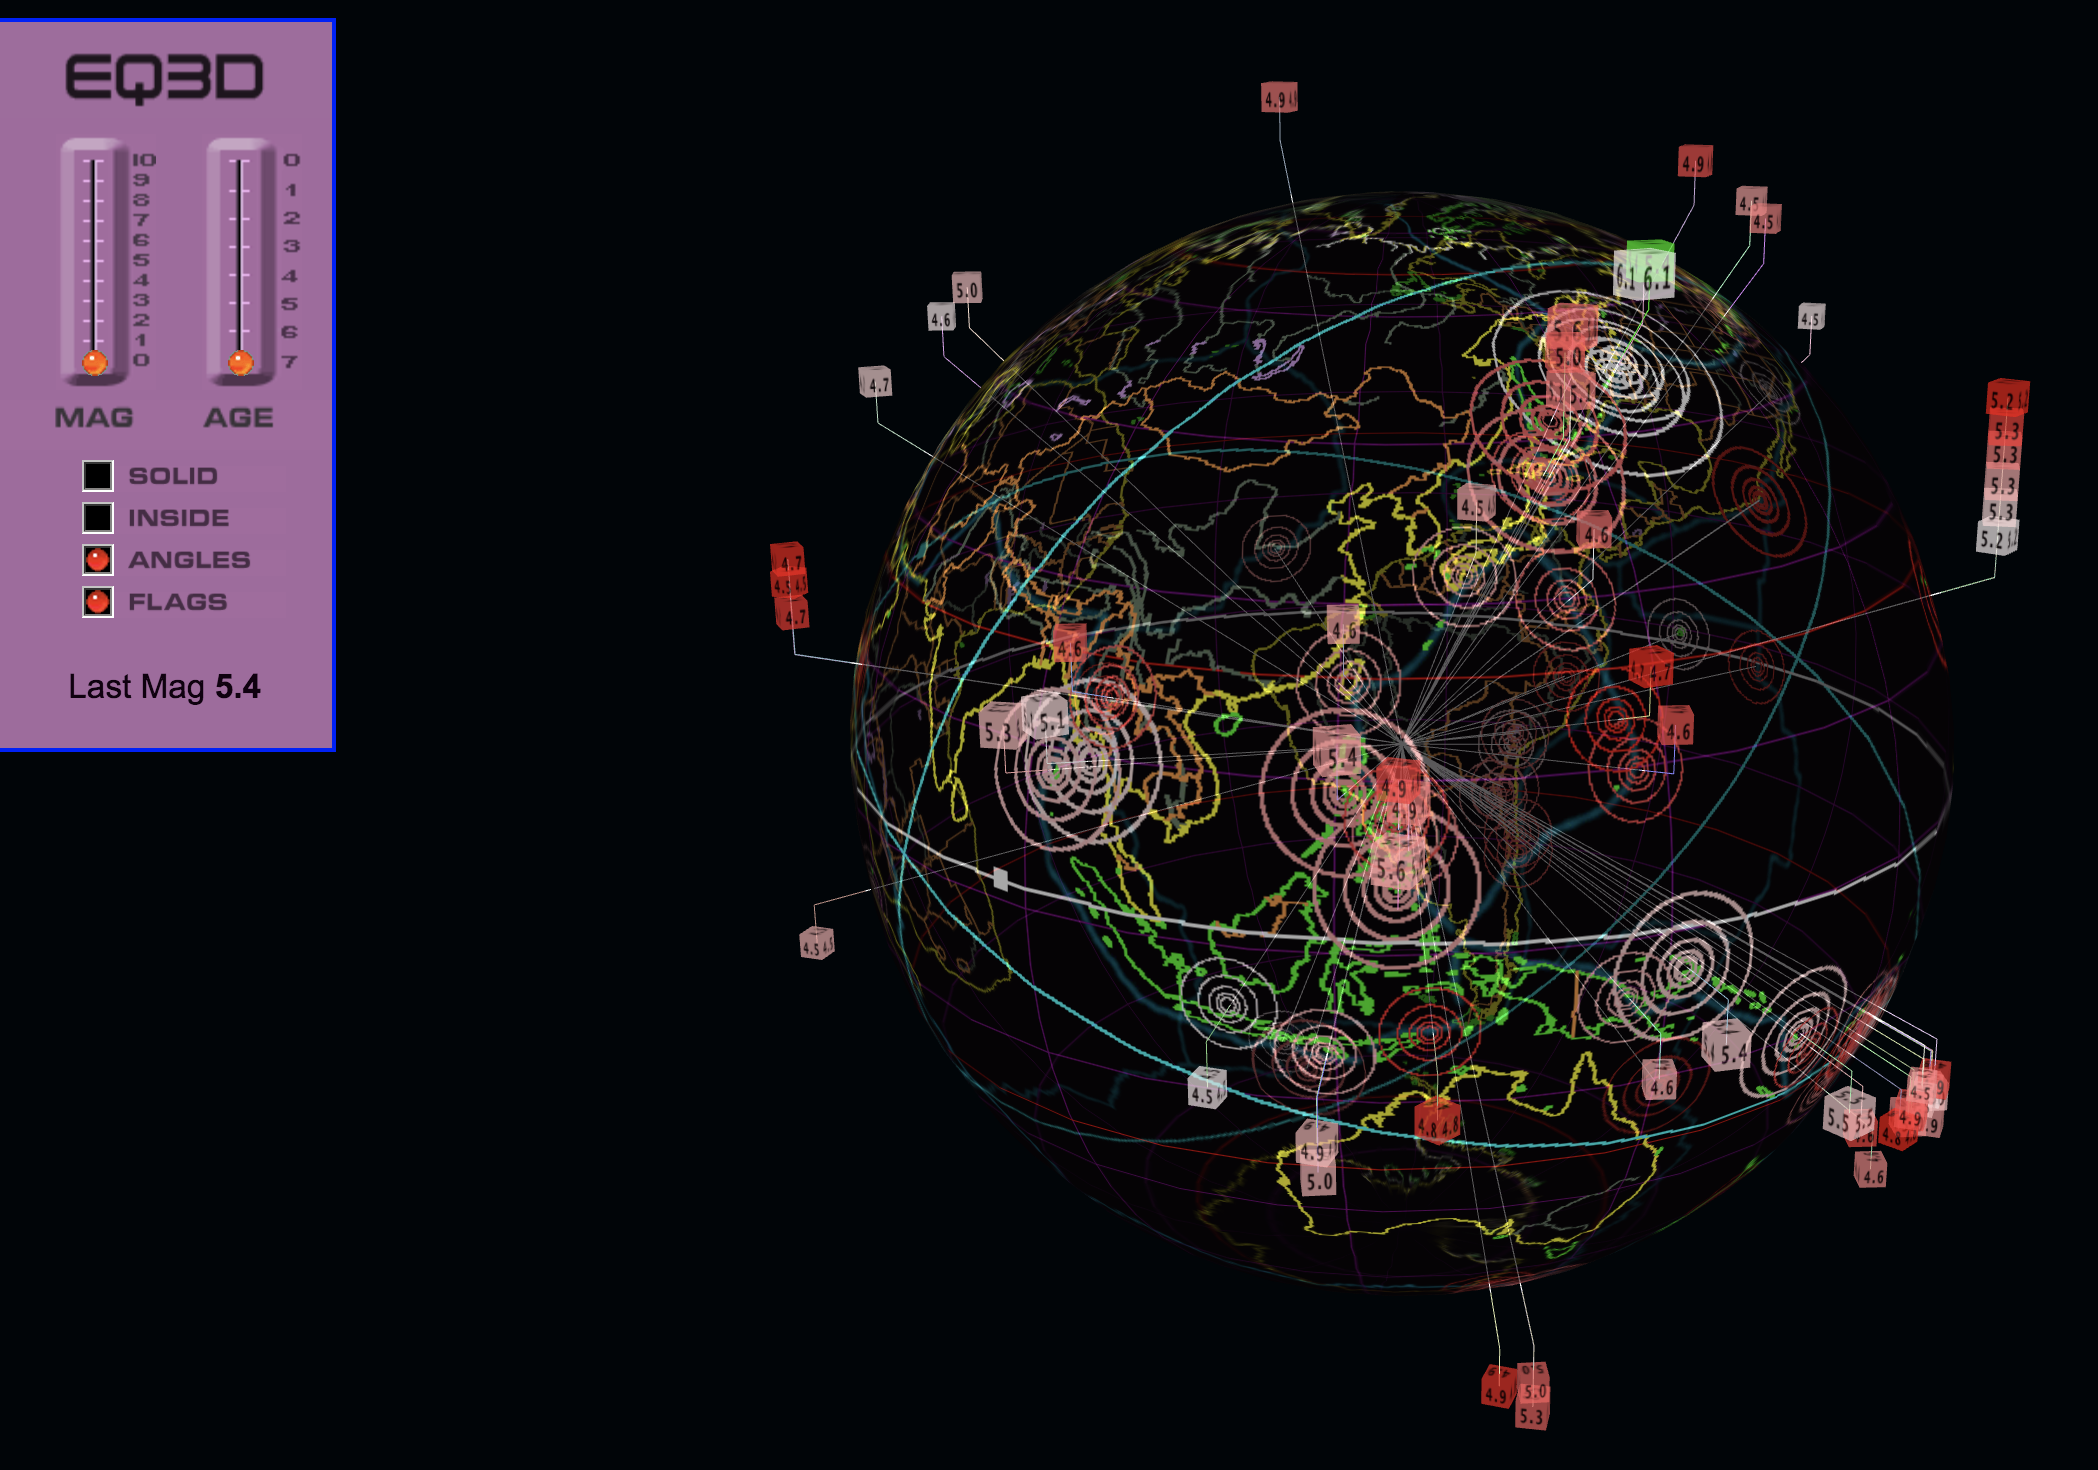
\includegraphics[width=0.8\linewidth]{Earthquakes.png}
\caption{EarthQuake 3D is a simple and easy to use desktop display of the world's last 20 significant earthquakes. You can zoom and spin your way around the globe while viewing earthquakes in three dimensions. See at a glance up to seven days of global earthquake activity.}
\end{figure}

%----------------------------------------------------------------------------------------

\end{column} % End of the first column

\begin{column}{\sepwid}\end{column} % Empty spacer column

\begin{column}{\twocolwid} % Begin a column which is two columns wide (column 2)

\begin{columns}[t,totalwidth=\twocolwid] % Split up the two columns wide column

\begin{column}{\onecolwid}\vspace{-.6in} % The first column within column 2 (column 2.1)

%----------------------------------------------------------------------------------------
%	MATERIALS
%----------------------------------------------------------------------------------------

\begin{block}{High Level Design}

%The following materials were required to complete the research:

\begin{itemize}
\item Sensors will be connected to microcontroller boards, which will be registered with IOT Core.
\item  IOT Core will handle messages passed from microcontrollers and will serve as an endpoint for collecting data for reporting interfaces (web front ends) as well as alerting mechanisms (CloudWatch alarms, for demo).
\item We will demo a few example scenarios of setups that will automatically respond in various events (i.e. flooding, earthquakes) and show that IOT services will allow for automated responses without human intervention.

\end{itemize}

The  minimum viable product scope:

\begin{enumerate}
\item Minimum viable product is the raspberry pi
\item Shake raspberry pi device will be  able to sense  potential threat.
\item Device will be able to connect to AWS IoT to log information.
\item Device will be able to notify the intended target when a natural disaster occurs.
\end{enumerate}

\end{block}

%----------------------------------------------------------------------------------------

\end{column} % End of column 2.1

\begin{column}{\onecolwid}\vspace{-.6in} % The second column within column 2 (column 2.2)

%----------------------------------------------------------------------------------------
%	METHODS
%----------------------------------------------------------------------------------------

\begin{block}{Methods}

Continuous integration/continuous deployment design, we will be able to continuously integrate changes made to our source code  and commit it to a main branch which would be hosted within a private git repository that AWS provides which is AWS CodeCommit.  After we commit new versions of the source code to CodeCommit, AWS CodePipeline which is a service that enables continuous integration and delivery will be triggered for execution of an automated workflow for continuous delivery of compiling, testing, and deploying the source code every time one member of our capstone team submits a new feature or version of the code to AWS CodeCommit. 

After this initial process, AWS CodePipeline will then send the updated version of the source code to AWS CodeBuild, which is a fully managed build service that handles the tasks responsible for compiling  and building the docker container image. 


\end{block}

%----------------------------------------------------------------------------------------

\end{column} % End of column 2.2

\end{columns} % End of the split of column 2 - any content after this will now take up 2 columns width

%----------------------------------------------------------------------------------------
%	IMPORTANT RESULT
%----------------------------------------------------------------------------------------

\begin{alertblock}{Motivation}

We want to build a device that can not only alerts individuals in their homes, but also be used nationwide with large organizations and federal agencies to provide an earlier response time in the event of larger natural disasters. We also hope to achieve some functionality with other IoT devices in which it can start carrying out the actions needed to suppress or eradicate the emergency in its entirety.  


\end{alertblock} 

%----------------------------------------------------------------------------------------

\begin{columns}[t,totalwidth=\twocolwid] % Split up the two columns wide column again

\begin{column}{\onecolwid} % The first column within column 2 (column 2.1)

%----------------------------------------------------------------------------------------
%	MATHEMATICAL SECTION
%----------------------------------------------------------------------------------------

\begin{block}{Visualization Results}

\begin{figure}
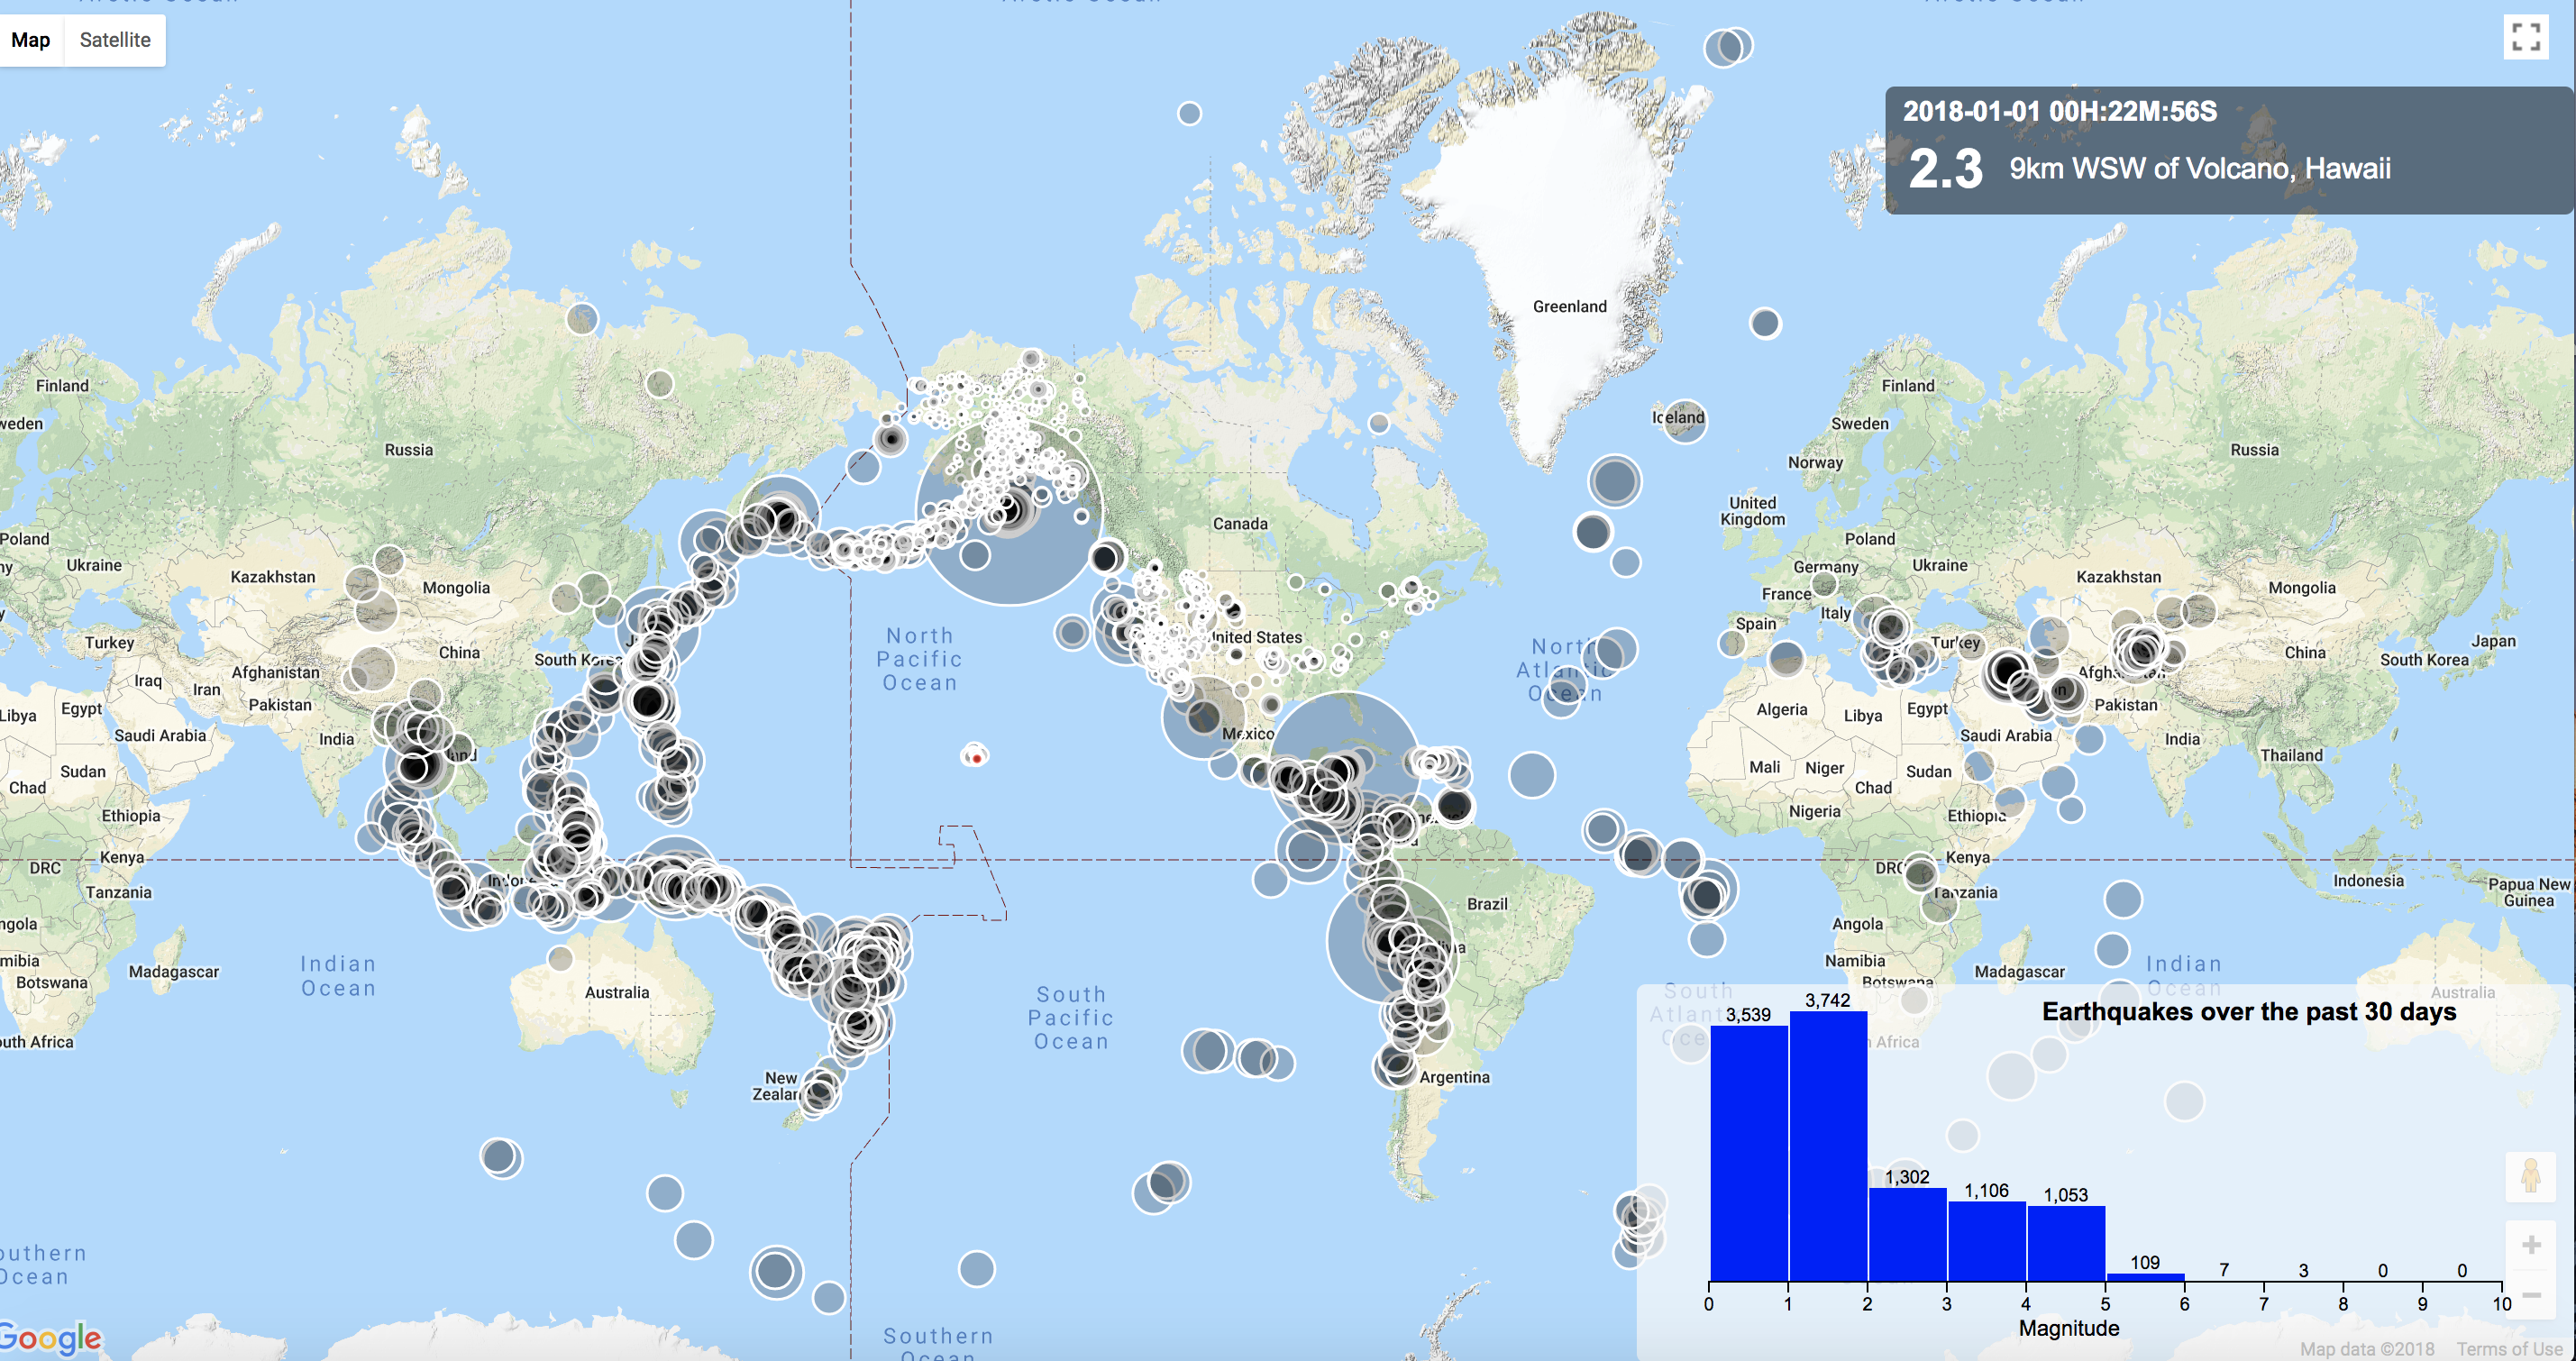
\includegraphics[width=0.8\linewidth]{Earthquake_Catalog.png}
\caption{Google Earth map that shows all seismicity around the world with ranging from Magnitude 1-10 on the richter scale. }
\end{figure}



\end{block}

%----------------------------------------------------------------------------------------

\end{column} % End of column 2.1

\begin{column}{\onecolwid} % The second column within column 2 (column 2.2)

%----------------------------------------------------------------------------------------
%	RESULTS
%----------------------------------------------------------------------------------------

\begin{block}{Visualization Results}

\begin{figure}
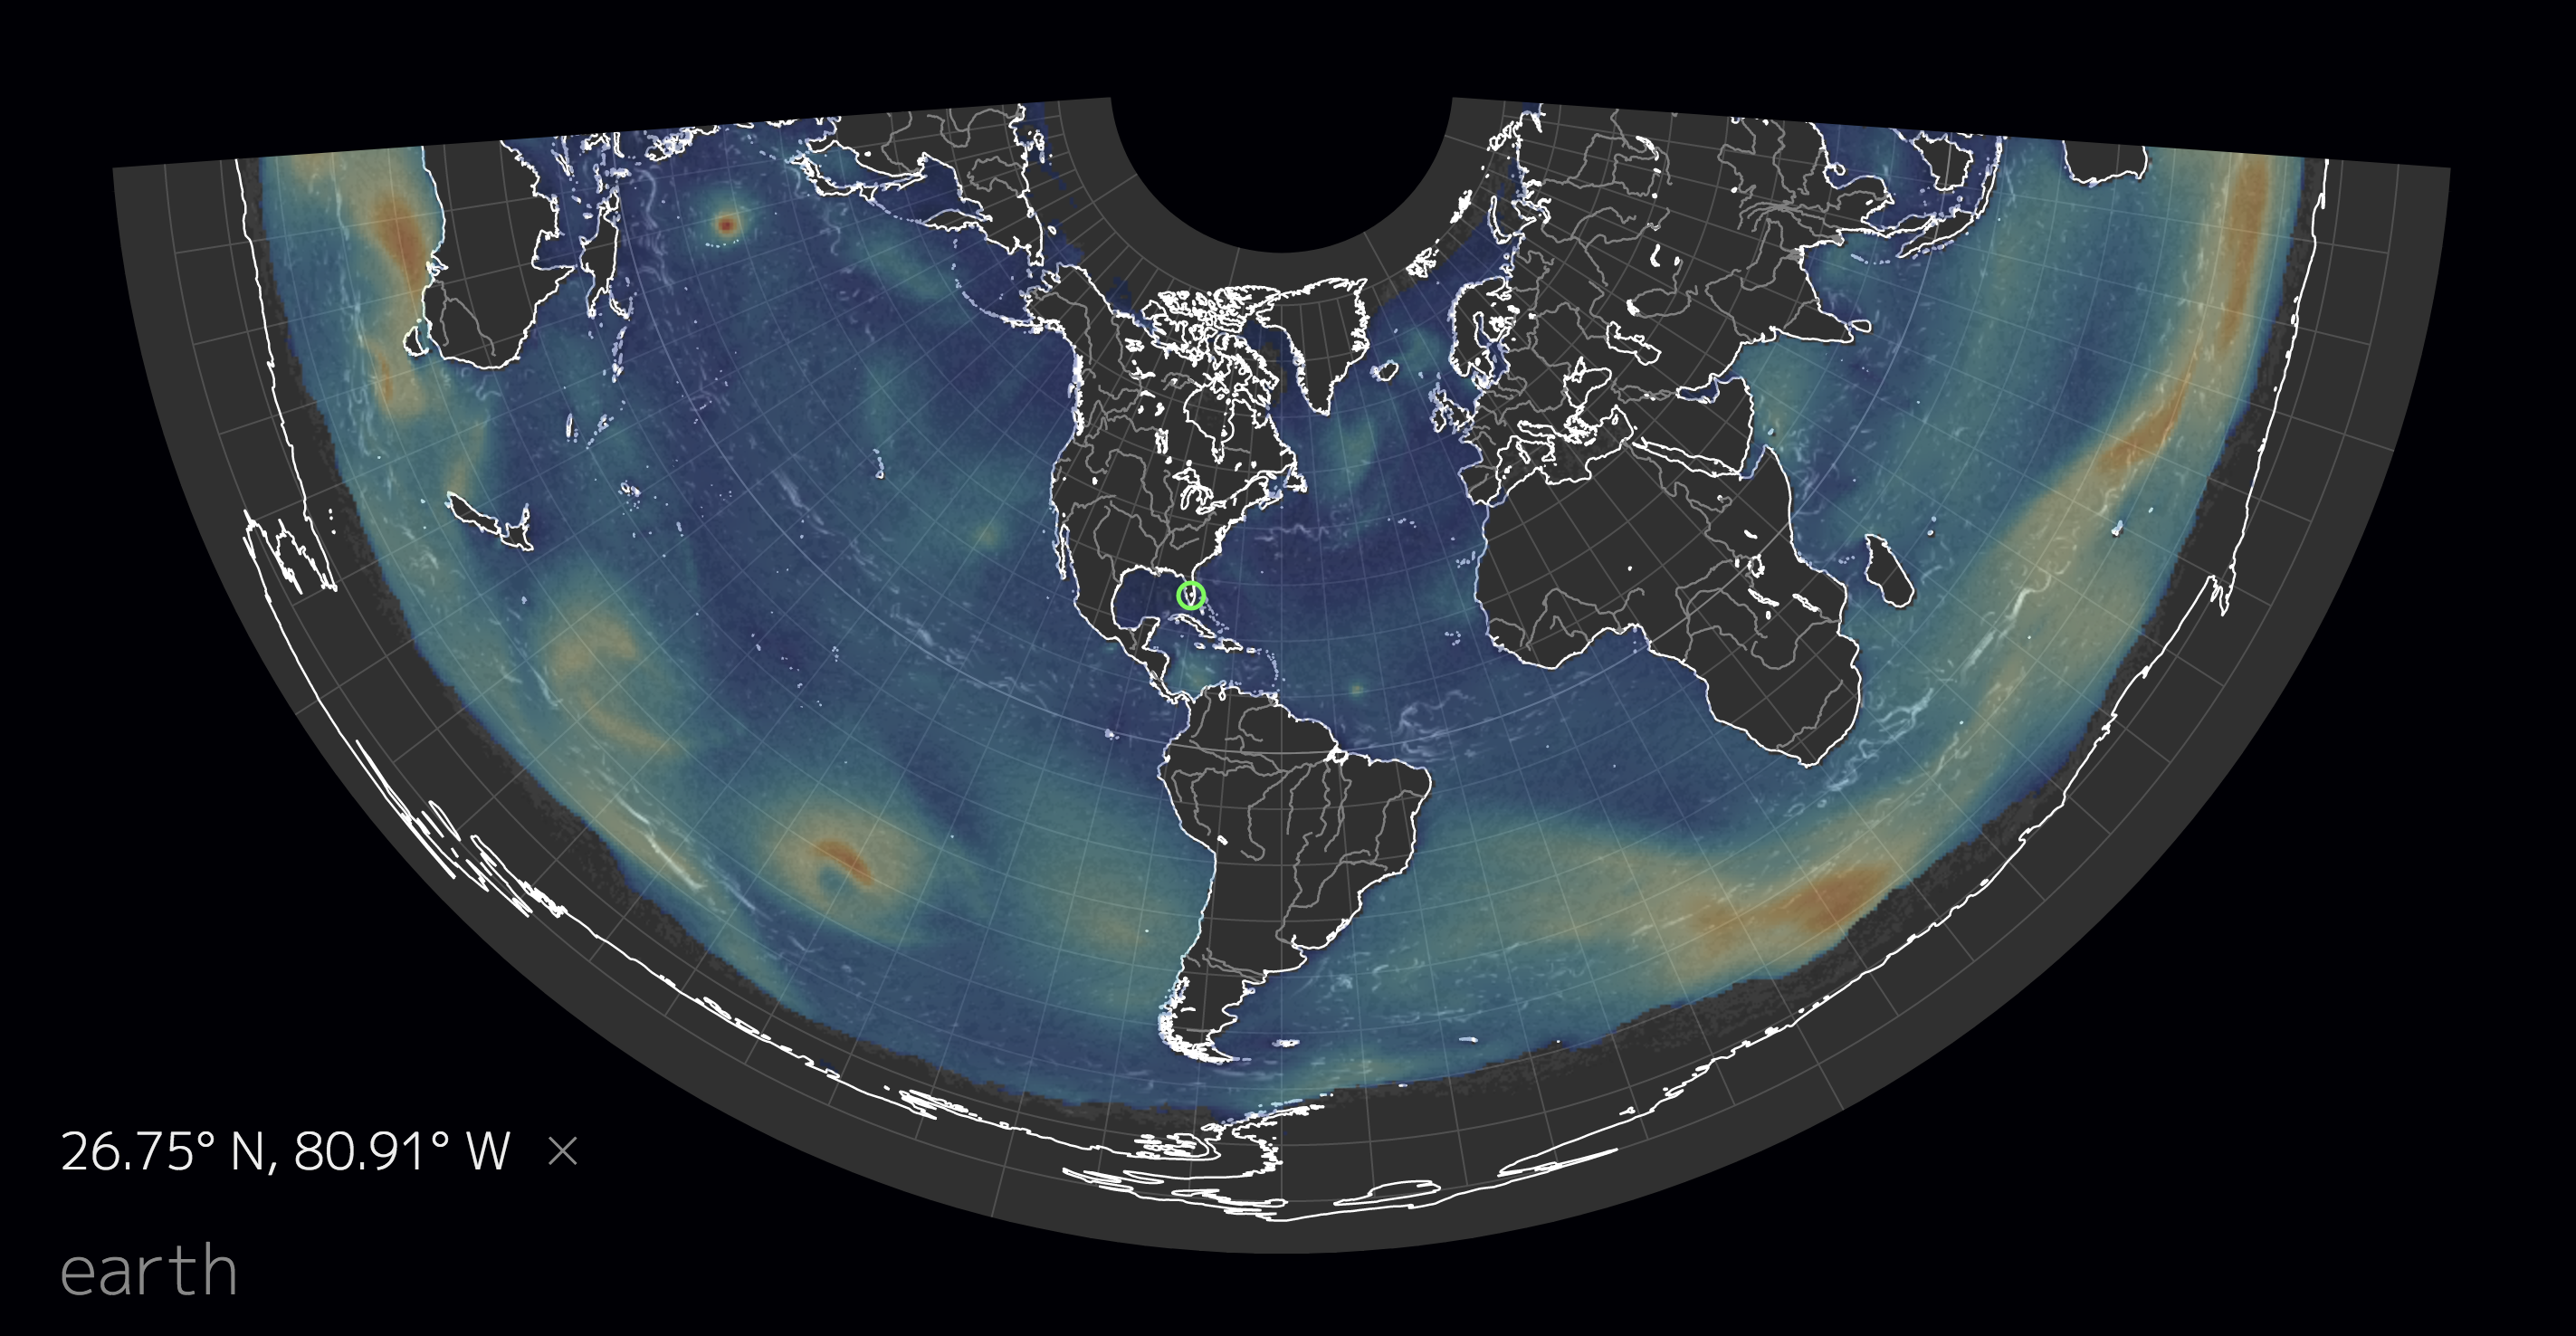
\includegraphics[width=0.8\linewidth]{Flood_Levels.png}
\caption{A visualization of global weather conditions
forecast by supercomputers
updated every three hours ocean surface current estimates
updated every five days.}
\end{figure}



\end{block}

%----------------------------------------------------------------------------------------

\end{column} % End of column 2.2

\end{columns} % End of the split of column 2

\end{column} % End of the second column

\begin{column}{\sepwid}\end{column} % Empty spacer column

\begin{column}{\onecolwid} % The third column

%----------------------------------------------------------------------------------------
%	CONCLUSION
%----------------------------------------------------------------------------------------

\begin{block}{Conclusion}

With ED2, we hope to achieve an emergency response device that can provide people the warning of an emergency before it is too late. The quicker the response time, the quicker individuals can prepare and find safety or slow/stop the emergency.   

\end{block}

%----------------------------------------------------------------------------------------
%	ADDITIONAL INFORMATION
%----------------------------------------------------------------------------------------

\begin{block}{Future Considerations}

For future considerations for the capstone would be  exploring the enhanced version of Earthquake 3D software tool which has the most up to date version of the program and contains more features than the free edition. The Earthquake 3D software can be install locally to Windows computer where a user can get a live feed up to 30 days of earthquake waveform data from multiple seismic networks like, USGS, EMSC, Geoscience, GeoNet, BGS, and Geophone. Also, the enhanced version of the Earthquake 3D software offers new features like Earthquake Alert Sounds, custom External Earth Images, and more.

\end{block}

%----------------------------------------------------------------------------------------
%	REFERENCES
%----------------------------------------------------------------------------------------

\begin{block}{References}

\nocite{*} % Insert publications even if they are not cited in the poster


\small{\bibliographystyle{unsrt}
\bibliography{sample}}


\begin{enumerate}
\item 3D Earthquake Software by Richard Wolton
\item Kilb, D. L., Peng, Z., Simpson, D., Michael, A. J., Fisher, M., \& Rohrlick, D. (2012). Listen, watch, learn: SeisSound video products. Seismological Research Letters, 83(2), 281-286. https://doi.org/10.1785/gssrl.83.2.281.
\item https://earth.nullschool.net/ (Interactive Weather Model)
\end{enumerate}
\end{block}

%----------------------------------------------------------------------------------------
%	ACKNOWLEDGEMENTS
%----------------------------------------------------------------------------------------

\setbeamercolor{block title}{fg=red,bg=white} % Change the block title color

\begin{block}{Acknowledgements}

\small{\rmfamily{We would like to thank Tech U program for their support and guidance with the capstone project. Special thanks and knowledgement to our mentor, Tim Wilson, Innovation Lab Product Manager for all the advice and expertise on the subject matter pertaining to the hardware component of our capstone project. }} \\

\end{block}

%----------------------------------------------------------------------------------------
%	CONTACT INFORMATION
%----------------------------------------------------------------------------------------

\setbeamercolor{block alerted title}{fg=black,bg=norange} % Change the alert block title colors
\setbeamercolor{block alerted body}{fg=black,bg=white} % Change the alert block body colors

\begin{alertblock}{Capstone Team}

\begin{itemize}
\item Adarsha Subick \textbf{Solutions Architect}
\item Sulaman Khan \textbf{Solutions Architect}
\item Lennox Thompson \textbf{Technical Trainer}
\end{itemize}

\end{alertblock}

\begin{center}
\begin{tabular}{ccc}

\includegraphics[width=0.4\linewidth]{logo.png} & \hfill & 
\includegraphics[width=0.4\linewidth]{logo.png}
\end{tabular}
\end{center}

%----------------------------------------------------------------------------------------

\end{column} % End of the third column

\end{columns} % End of all the columns in the poster

\end{frame} % End of the enclosing frame

\end{document}
